\documentclass[12pt,a4paper]{article}
\usepackage[utf8]{inputenc}
\usepackage[T1]{fontenc}
\usepackage[brazil]{babel}
\usepackage[margin=2.5cm]{geometry}
\usepackage{graphicx}
\usepackage{fancyhdr}
\usepackage{float}
\usepackage{geometry}

\begin{document}

\pagestyle{fancy}
\fancyhf{}
\lhead{\textbf{Universidade de Rio Verde - UniRV}\\ Disciplina: Banco de Dados}
\rhead{Data: \_\_\_/\_\_\_/\_\_\_\_\\ Aluno(a): \makebox[6cm]{\hrulefill}}

\vspace*{0.5cm}
 
\begin{center}
    {\Large \textbf{Atividade Prática: Criação de Tabelas (SQL DDL)}}
\end{center}

\vspace{0.5cm}

\noindent \textbf{Objetivo:} Escrever a linguagem de definição de dados (DDL) em SQL para criar a base de dados a partir dos Diagramas Entidade-Relacionamento (DER) fornecidos. \\

\noindent \textbf{Instruções:} Para cada um dos diagramas apresentados a seguir, construa os comandos SQL (\texttt{CREATE TABLE}) necessários. Preste atenção aos seguintes detalhes:
\begin{itemize}
    \item Nomeação correta de tabelas e colunas;
    \item Definição de Tipos de Dados adequados;
    \item Identificação e especificação de Chaves Primárias (\texttt{PRIMARY KEY});
    \item Identificação e especificação de Chaves Estrangeiras (\texttt{FOREIGN KEY}), observando as cardinalidades para saber onde posicioná-las;
    \item Uso de restrições de obrigatoriedade (\texttt{NOT NULL}) quando julgar necessário.
\end{itemize}

\vspace{0.5cm}
\hrule
\vspace{0.5cm}

% Exercício 1
\section*{Exercício 1}
Escreva as sentenças SQL para criar as tabelas relativas ao seguinte diagrama:

\begin{figure}[H]
    \centering
    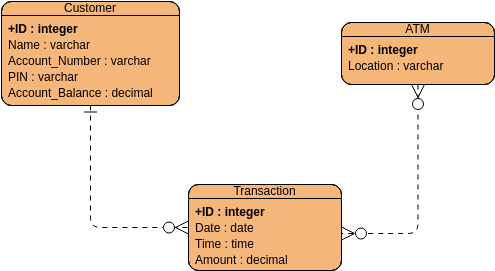
\includegraphics[width=0.8\textwidth]{erd1.png}
    \caption{Diagrama 1}
\end{figure}

\vspace{0.5cm}
\noindent \textbf{Comandos SQL:}
\vspace{5cm}

\
% Exercício 2
\section*{Exercício 2}
Escreva as sentenças SQL para criar as tabelas relativas ao seguinte diagrama:

\begin{figure}[H]
    \centering
    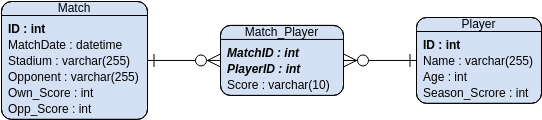
\includegraphics[width=0.8\textwidth]{erd2.png}
    \caption{Diagrama 2}
\end{figure}

\vspace{0.5cm}
\noindent \textbf{Comandos SQL:}
\vspace{5cm}

\
% Exercício 3
\section*{Exercício 3}
Escreva as sentenças SQL para criar as tabelas relativas ao seguinte diagrama:

\begin{figure}[H]
    \centering
    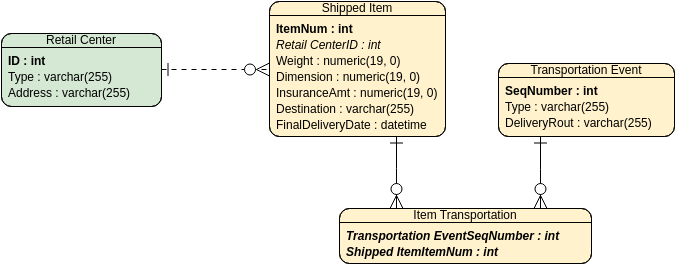
\includegraphics[width=0.8\textwidth]{erd3.png}
    \caption{Diagrama 3}
\end{figure}

\vspace{0.5cm}
\noindent \textbf{Comandos SQL:}
\vspace{5cm}

\
% Exercício 4
\section*{Exercício 4}
Escreva as sentenças SQL para criar as tabelas relativas ao seguinte diagrama:

\begin{figure}[H]
    \centering
    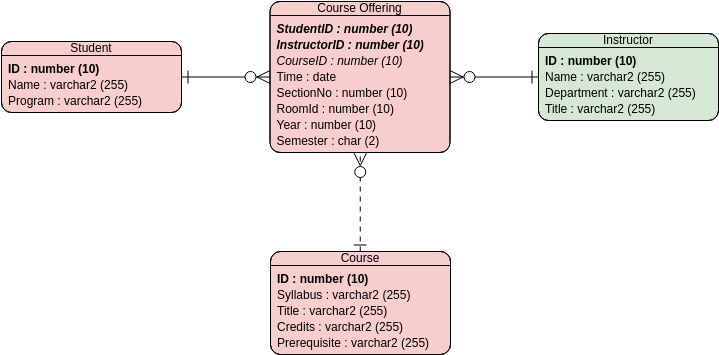
\includegraphics[width=0.8\textwidth]{erd4.png}
    \caption{Diagrama 4}
\end{figure}

\vspace{0.5cm}
\noindent \textbf{Comandos SQL:}
\vspace{5cm}

\
% Exercício 5
\section*{Exercício 5}
Escreva as sentenças SQL para criar as tabelas relativas ao seguinte diagrama:

\begin{figure}[H]
    \centering
    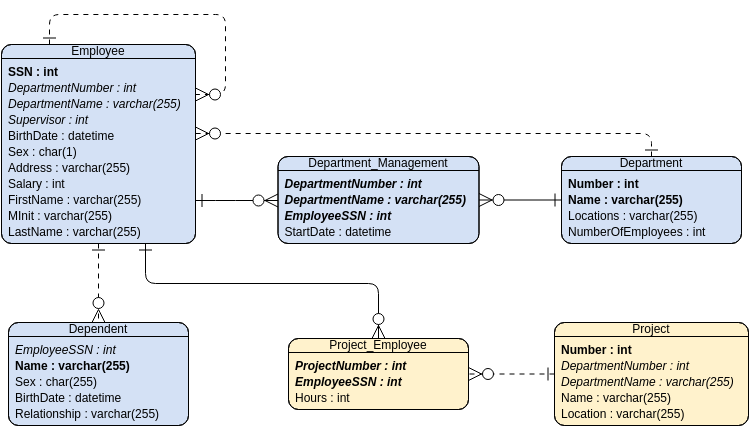
\includegraphics[width=0.8\textwidth]{erd5.png}
    \caption{Diagrama 5}
\end{figure}

\vspace{0.5cm}
\noindent \textbf{Comandos SQL:}
\vspace{5cm}

\
% Exercício 6
\section*{Exercício 6}
Escreva as sentenças SQL para criar as tabelas relativas ao seguinte diagrama:

\begin{figure}[H]
    \centering
    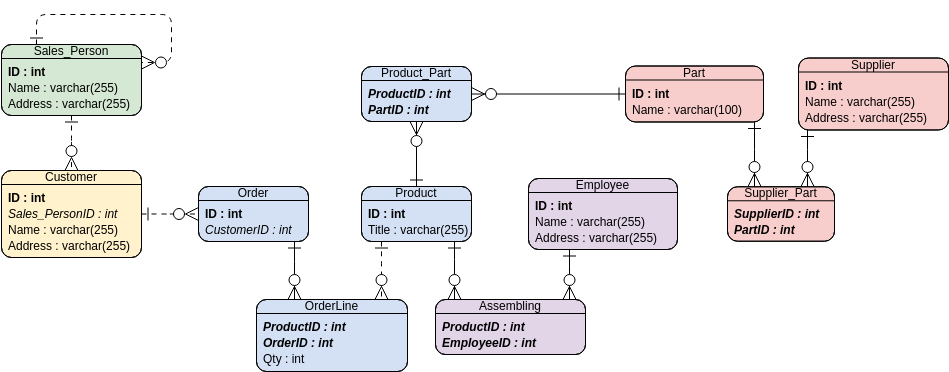
\includegraphics[width=0.8\textwidth]{erd6.png}
    \caption{Diagrama 6}
\end{figure}

\vspace{0.5cm}
\noindent \textbf{Comandos SQL:}
\vspace{5cm}

\end{document}
